\scanpage{88}
\mspage{1}
% archive foliation: 87
$\mathfrak X$ schéma formel régulier, \inserted{connexe},
$\mathfrak X_0=X_0$ diviseur régulier,
$D=\deleted{\unsure{+}}\bigcup_0^{\unsure{r}}D_i$,
\unsure{diviseurs} \deleted{avec} \unsure{normaux}
croisant normalement $D_0=X_0$,
[les $D_i$ réguliers irréductibles]
$D'=\sum_{i\ne0}D_i$, $\unsure{D'_0|D_0}$ induit sur $X_0$.

\diagram{
\begin{tikzcd}[column sep=small]
e\arrow[r]&\overline I_0\arrow[r]&
\pi_1^t(\mathfrak X/D,\bar\xi_1)\arrow[r]&
\pi_1^t(X_0/D'_0,\bar\xi_0)\arrow[r]&e\\
&&\text{''}&\text{''}\quad\text{''}&\\
&&\pi_1^t(\mathfrak X/D)&
\pi_1^t(U)\quad\pi_1(\mathfrak X/D',\bar\xi_0)&\\
&&&\text{''}&\\
&&&D_0-D'_0&
\end{tikzcd}
}
\margin{\figure{
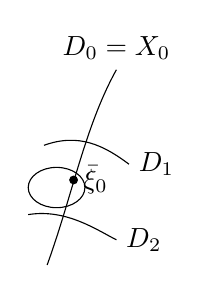
\begin{tikzpicture}[scale=.8]
\draw (0,0) .. controls (.4,1.1) and (.6,2.2) .. (1.1,3.1)
 node[above]{$D_0=X_0$};
\draw (-.05,1.9)..controls(.5,2.1)and(.9,1.9)..(1.3,1.6)node[right]{$D_1$};
\draw (-.3,.8)..controls(.3,.9)and(.8,.55)..(1.1,.4)node[right]{$D_2$};
\fill (.42,1.35)circle(2pt);
\node[right]at(.42,1.35){$\bar\xi_0$};
\draw (.15,1.23)ellipse(.45 and .32);
\end{tikzpicture}
}}

\[
\deleted{\unsure{\mu}\longrightarrow}
\mu^\infty_{X_0,\mathrm{tame}}(\bar\xi_0)
\longrightarrow I_0\longrightarrow0
\]
\[
\begin{array}{c}
\text{''}\\[-2pt]
\mu(\deleted{\unsure{\bar\xi}}\bar\xi_0)
\end{array}
\]
\margin{$=\varprojlim_{\substack{n>0\\n\text{ inversible dans }\underline O_{X_0}}}\mu_n$}

\margin{\diagram{
\begin{tikzcd}
\mu\arrow[r]&I\arrow[r]&0\\
\mu^\infty_{X_0,\mathrm{tame}}\arrow[u,phantom,"\text{''}"]&&
\end{tikzcd}
}
faisceaux étales sur $X_0$}

Donc
\[
\prod_{\ell\underline O_{X_0}=\underline O_{X_0}}\mathbf Z_\ell
\]
\[
\mu(\bar\xi_0)\longrightarrow\pi_1^t(\mathfrak X/D)
\longrightarrow\pi_1^t(U)\longrightarrow e
\]
Opérations de $\pi_1^t(U)$ sur $I_0$ via opérations de
$\pi_1^t(U)$ sur \deleted{$I$}$\mu$
\deleted{\unsure{via op---}}.
L'extension décrite par
\[
\alpha\deleted{\unsure{\xi}}\in H^2(\pi_1^t(U),I_0)
\qquad
\deleted{\unsure{\xi}}\alpha=?
\]

\uline{Lemme 1} Soit $\widetilde U^t$ rev. étale de $U$ défini par
$\pi_1^t$. Alors
\[
H^1(\widetilde U^t,J)=0
\quad\text{si }J\text{ premier aux car. résiduelles de }X_0
\]
[p. ex. $J=I$].
\margin{constant}
\margin{for all $H^i$, $i>0$, true if $D_0$ is \uline{curve}
\uline{over a field}}

\diagram{
\begin{tikzcd}[column sep=small]
0\arrow[r]&H^2(\pi_1^t,I)\arrow[r,"\rho"]&
H^2(U,I)\arrow[r]&
H^2(\widetilde U^t,I_0)^{\pi_1^t}\arrow[r]&
H^3(\pi_1^t,I)\arrow[d]\\
&&&&H^3(U,I)
\end{tikzcd}
}
\margin{constant sur $\widetilde U^t$}
\[
\begin{array}{c}
\unsure{\simeq}\\
\operatorname{Hom}(\pi_2(\widetilde U^t),I)^{\pi_1^t}\\
\operatorname{Hom}(\pi_2^t(U),I)^{\pi_1^t}
\end{array}
\]
\margin{Serre--Hochschild
\[
H^{\unsure{n}}(U,J)\Longleftarrow
H^p(\pi_1^t,H^q(\widetilde U^t,J))
\]
\deleted{\unsure{$\rho$}} \unsure{can.}
}

Donc $\alpha$ connu qd on connaît
$\rho(\alpha)$, et l'image de plus dans
\[
H^2(\widetilde U^t,I)^{\pi_1^t}
\simeq\operatorname{Hom}(\unsure{\pi_1^t(U)|\pi_2^t(U)},I)^{\pi_1^t}
\]
est nulle.
